\clearpage\newpage
\subsection{Navigational map}

This is the sitemap of the app, it shows how it can be navigated. It consists of boxes representing the screens and arrows with icons as labels that represent the button that navigates to the corresponding page. The empty arrows mean that the user can go back, either by pressing the back button of the browser, or the back button of the app. 

This map aims to be as simple as possible, to be easier to navigate by the users. To achieve that, the \textit{Dashboard/Welcome} and \textit{Login/Logout} screens are merged into one. Moreover, the \textit{Edit subject}, \textit{Edit \& add subject} and \textit{Create subject} screens look practically the same, so when the user learns how to use one, the gained knowledge can be applied to the other screens.

\vfill
\begin{figure}[ht!]
    \center
    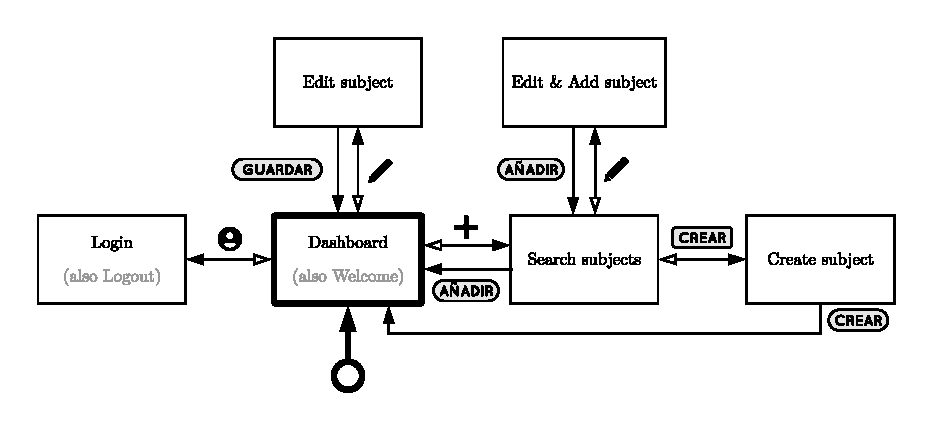
\includegraphics[width=1\columnwidth]{media/diagrams/navigation.pdf}
    \caption{Navigation diagram}
    \label{fig:ux_diagram}
\end{figure}
\vfill